\documentclass[aspectratio=169,10pt]{beamer}

% Compile from this directory with:
%   latexmk -pdf hlcv_project_slides.tex

\usepackage[T1]{fontenc}
\usepackage[utf8]{inputenc}
\usepackage{lmodern}
\usepackage{array}
\usepackage{booktabs}
\usepackage{graphicx}
\usepackage{tabularx}
\usepackage{tikz}
\usetikzlibrary{arrows.meta,positioning}

\definecolor{forest}{HTML}{173F35}
\definecolor{leaf}{HTML}{2F7D6B}
\definecolor{gold}{HTML}{E5A84B}
\definecolor{coral}{HTML}{C95746}
\definecolor{ink}{HTML}{1D2528}
\definecolor{muted}{HTML}{64706F}
\definecolor{paper}{HTML}{F6F3EB}
\definecolor{palegreen}{HTML}{E7F0EC}
\definecolor{palegold}{HTML}{F8EDD7}

\setbeamertemplate{navigation symbols}{}
\setbeamercolor{normal text}{fg=ink,bg=white}
\setbeamercolor{frametitle}{fg=forest,bg=white}
\setbeamercolor{title}{fg=forest}
\setbeamercolor{subtitle}{fg=muted}
\setbeamercolor{structure}{fg=leaf}
\setbeamercolor{block title}{fg=white,bg=forest}
\setbeamercolor{block body}{fg=ink,bg=paper}
\setbeamerfont{frametitle}{series=\bfseries,size=\Large}
\setbeamerfont{title}{series=\bfseries,size=\LARGE}
\setbeamertemplate{itemize item}{\color{leaf}$\blacktriangleright$}
\setbeamertemplate{itemize subitem}{\color{gold}$\bullet$}

\setbeamertemplate{footline}{
  \leavevmode%
  \hbox{%
    \begin{beamercolorbox}[wd=.84\paperwidth,ht=2.5ex,dp=1ex,leftskip=1.2em]{author in head/foot}%
      \color{muted}\scriptsize HLCV Final Project \textbullet\ Boundary-Aware Field Segmentation
    \end{beamercolorbox}%
    \begin{beamercolorbox}[wd=.16\paperwidth,ht=2.5ex,dp=1ex,center]{date in head/foot}%
      \color{muted}\scriptsize \insertframenumber/\inserttotalframenumber
    \end{beamercolorbox}%
  }%
}

\newcommand{\source}[1]{%
  \vfill
  {\color{muted}\fontsize{5.7}{6.5}\selectfont Source: #1\par}
}
\newcommand{\config}[1]{\texttt{\footnotesize #1}}
\newcommand{\pill}[2]{%
  \tikz[baseline=(n.base)]\node[
    fill=#1,rounded corners=2pt,inner xsep=6pt,inner ysep=3pt
  ] (n) {\strut #2};%
}
\title{Boundary-Aware Agricultural Field Segmentation}
\subtitle{Comparing auxiliary distance, direct weighting, and explicit boundary prediction}
\author{HLCV Team 004}
\institute{Saarland University}
\date{July 2026}

\begin{document}

\begin{frame}
  \titlepage
  \vspace{-0.9em}
  \begin{center}
    \pill{palegreen}{Four controlled methods}
    \hspace{0.45em}
    \pill{palegold}{1,430 held-out test chips}
  \end{center}
\end{frame}

\begin{frame}{The challenge is preserving individual fields, not only field area}
  \begin{columns}[T,onlytextwidth]
    \begin{column}{0.69\textwidth}
      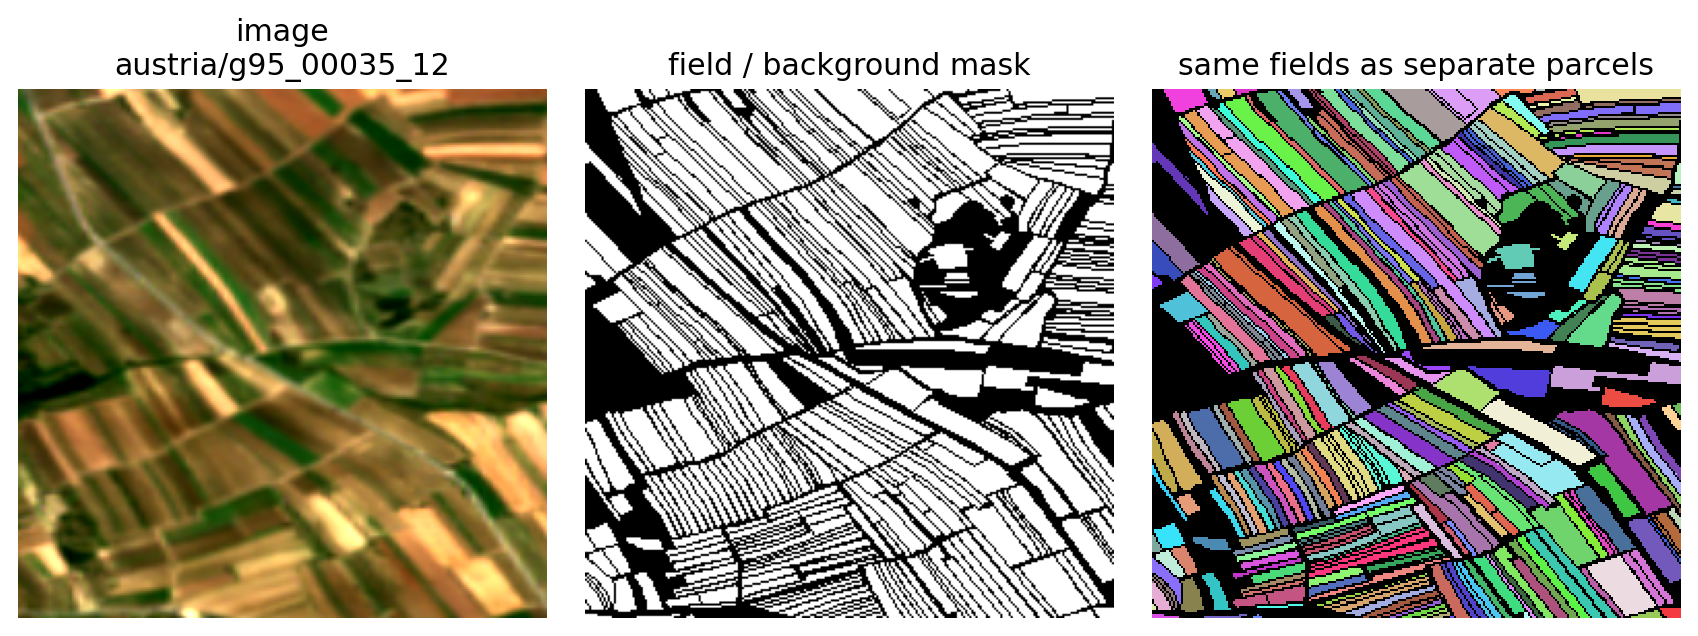
\includegraphics[
        width=\textwidth,
        height=0.70\textheight,
        keepaspectratio
      ]{../Visualizations/problem_setup/val_blob_issue.png}
    \end{column}
    \begin{column}{0.28\textwidth}
      \vspace{0.5em}
      \begin{block}{Failure mode}
        A binary mask can cover the correct area while merging neighboring fields.
      \end{block}
      \vspace{0.6em}
      \begin{block}{Project goal}
        Improve border agreement without sacrificing region overlap.
      \end{block}
    \end{column}
  \end{columns}
  \source{FTW imagery and labels; visualization generated in this project.}
\end{frame}

\begin{frame}{Data and supervision}
  \begin{columns}[T,onlytextwidth]
    \begin{column}{0.47\textwidth}
      \begin{block}{Fields of The World subset}
        \begin{tabularx}{\textwidth}{@{}>{\bfseries}lX@{}}
          Countries & Austria, Croatia, Denmark \\
          Input & two seasonal images, each with RGB+NIR (8 channels total) \\
          Resolution & $256\times256$ pixels; 10 m per pixel \\
          Labels & field mask + FTW instance mask \\
        \end{tabularx}
      \end{block}
      \vspace{0.45em}
      \begin{center}
        \pill{palegreen}{10,938 train}
        \quad
        \pill{paper}{1,347 validation}
        \quad
        \pill{palegold}{1,430 test}
      \end{center}
    \end{column}
    \begin{column}{0.49\textwidth}
      \begin{block}{How the labels are used}
        \textbf{Binary field mask}\hfill
        {\color{leaf}\bfseries Mask head}\\[-0.05em]
        \small Direct target: field or background at every pixel.

        \vspace{0.45em}
        {\color{muted}\rule{\linewidth}{0.35pt}}
        \vspace{0.35em}

        \textbf{FTW instance mask}\\[-0.05em]
        \small Provided by the dataset; separates neighboring fields.

        \vspace{0.25em}
        \centering
        {\color{muted}\small converted into $\Downarrow$}
        \par
        \raggedright
        \textbf{Signed distance field (SDF)}\hfill
        {\color{leaf}\bfseries Distance head}\\[-0.05em]
        \small Derived target: distance to the nearest field boundary.
      \end{block}
    \end{column}
  \end{columns}
  \source{Kerner et al., ``Fields of The World,'' AAAI 2025.}
\end{frame}

\begin{frame}{Related work and what we contributed}
  \begin{columns}[T,onlytextwidth]
    \begin{column}{0.47\textwidth}
      \begin{block}{Built upon}
        \begin{itemize}
          \item \textbf{FTW}: global, multi-date Sentinel-2 field benchmark.
          \item \textbf{U-Net}: encoder--decoder with skip connections for dense prediction.
          \item \textbf{Distance-aware supervision}: geometry can complement region losses.
        \end{itemize}
      \end{block}
    \end{column}
    \begin{column}{0.49\textwidth}
      \begin{block}{Our project work}
        \begin{itemize}
          \item Added an instance-derived SDF target and a second regression head.
          \item Added an SDF-based weighting map to focus BCE near field borders.
          \item Added an explicit boundary-prediction head and compared all checkpoints on the test set.
        \end{itemize}
      \end{block}
    \end{column}
  \end{columns}
  \vspace{0.55em}
  \centering
  \pill{palegold}{Research question: where should boundary information enter the learning objective?}
  \source{Ronneberger et al., MICCAI 2015; Kervadec et al., MIDL 2019 / MedIA 2021.}
\end{frame}

\begin{frame}{Four methods, one controlled comparison}
  \small
  \setlength{\tabcolsep}{4pt}
  \renewcommand{\arraystretch}{1.22}
  \begin{tabularx}{\textwidth}{@{}
    >{\raggedright\arraybackslash}p{0.18\textwidth}
    >{\raggedright\arraybackslash}p{0.20\textwidth}
    >{\raggedright\arraybackslash}p{0.36\textwidth}
    >{\raggedright\arraybackslash}X@{}}
    \toprule
    \textbf{Method} & \textbf{Architecture} & \textbf{Training loss} & \textbf{Boundary signal} \\
    \midrule
    Mask baseline &
    one mask head &
    $\mathcal{L}_{BCE}+\mathcal{L}_{Dice}$ &
    none \\
    \addlinespace
    Two-head SDF &
    mask + distance heads &
    $\mathcal{L}_{BCE}+\mathcal{L}_{Dice}+0.1\mathcal{L}_{SDF}$ &
    auxiliary geometry \\
    \addlinespace
    Boundary BCE &
    one mask head &
    $\mathcal{L}_{WBCE}+\mathcal{L}_{Dice}$ &
    direct mask gradients \\
    \addlinespace
    Mask + boundary &
    two active heads &
    $\mathcal{L}_{WBCE}+\mathcal{L}_{Dice}+2\mathcal{L}_{Bnd}$ &
    mask gradients + explicit border task \\
    \bottomrule
  \end{tabularx}

  \vspace{0.5em}
  \begin{columns}[T,onlytextwidth]
    \begin{column}{0.49\textwidth}
      \begin{block}{Held constant}
        Data, augmentation, U-Net width, optimizer, and evaluation code.
      \end{block}
    \end{column}
    \begin{column}{0.49\textwidth}
      \begin{block}{Checkpoint audit}
        The trained mask baseline uses ordinary \textbf{BCE + Dice}.
      \end{block}
    \end{column}
  \end{columns}
\end{frame}

\begin{frame}{Method 1: a second head predicts signed distance}
  \begin{columns}[T,onlytextwidth]
    \begin{column}{0.55\textwidth}
      \centering
      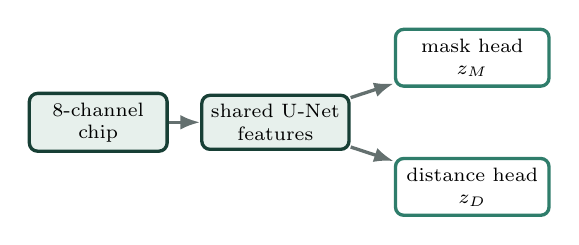
\begin{tikzpicture}[
        font=\scriptsize,
        box/.style={draw=forest,very thick,rounded corners=3pt,fill=palegreen,
          minimum width=1.75cm,minimum height=0.68cm,align=center},
        head/.style={draw=leaf,very thick,rounded corners=3pt,fill=white,
          minimum width=1.95cm,minimum height=0.68cm,align=center},
        arr/.style={-{Latex[length=2.5mm]},very thick,draw=muted}
      ]
        \node[box] (input) at (0,0) {8-channel\\chip};
        \node[box] (unet) at (2.25,0) {shared U-Net\\features};
        \node[head] (mask) at (4.75,0.82) {mask head\\$z_M$};
        \node[head] (sdf) at (4.75,-0.82) {distance head\\$z_D$};
        \draw[arr] (input) -- (unet);
        \draw[arr] (unet) -- (mask);
        \draw[arr] (unet) -- (sdf);
      \end{tikzpicture}

      \vspace{0.55em}
      \begin{block}{Joint objective}
        \footnotesize
        \[
          \begin{aligned}
            \mathcal{L}_{2H}
            &= \mathcal{L}_{BCE}(z_M,Y)
             + \mathcal{L}_{Dice}(\sigma(z_M),Y)\\
            &\quad + 0.1\,\mathrm{SmoothL1}(\tanh(z_D),D)
          \end{aligned}
        \]
      \end{block}
    \end{column}
    \begin{column}{0.41\textwidth}
      \begin{block}{Hypothesis}
        The SDF task forces shared features to encode individual field geometry.
      \end{block}
      \vspace{0.45em}
      \begin{itemize}
        \item $D>0$: inside an individual field
        \item $D\approx0$: field boundary
        \item $D<0$: background
        \item Inference still uses the mask head
      \end{itemize}
      \vspace{0.45em}
      \pill{palegreen}{+9,313 parameters}
      \quad
      \pill{paper}{+0.12\%}
    \end{column}
  \end{columns}
\end{frame}

\begin{frame}{Method 2: put boundary emphasis directly into BCE}
  \begin{columns}[T,onlytextwidth]
    \begin{column}{0.57\textwidth}
      \begin{block}{Boundary-weighted BCE}
        \small
        \[
          \mathcal{L}_{WBCE}
          = \frac{\sum_i w_i\,\mathrm{BCE}(z_i,y_i)}{\sum_i w_i}
        \]
        \vspace{-0.8em}
        \[
          w_i = 1 + 20\exp\!\left(-\frac{|D_i|}{0.12}\right)
        \]
      \end{block}
      \vspace{0.45em}
      \[
        \mathcal{L}_{final}
        = \mathcal{L}_{WBCE}+\mathcal{L}_{Dice}
      \]
      \small
      Dice preserves global region overlap; weighted BCE changes which pixel errors dominate the gradient.
    \end{column}
    \begin{column}{0.39\textwidth}
      \begin{block}{Pixel weight by distance}
        \centering
        \begin{tabular}{@{}lc@{}}
          \toprule
          $|D|$ & BCE weight \\
          \midrule
          $0$ & $\mathbf{21.0}$ \\
          $0.12$ & $8.36$ \\
          $0.24$ & $3.71$ \\
          far from border & $\approx1.0$ \\
          \bottomrule
        \end{tabular}
      \end{block}
      \vspace{0.55em}
      \begin{block}{Key difference}
        The boundary signal acts on the \textbf{final mask output}, not through an auxiliary task.
      \end{block}
    \end{column}
  \end{columns}
\end{frame}

\begin{frame}{Method 3: a second head predicts boundary pixels}
  \begin{columns}[T,onlytextwidth]
    \begin{column}{0.55\textwidth}
      \centering
      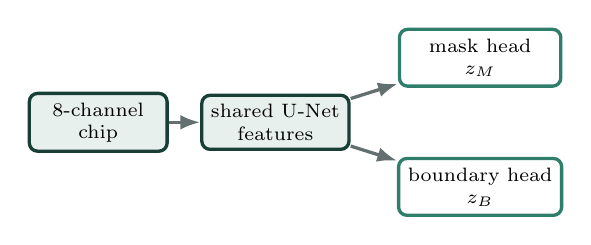
\begin{tikzpicture}[
        font=\scriptsize,
        box/.style={draw=forest,very thick,rounded corners=3pt,fill=palegreen,
          minimum width=1.75cm,minimum height=0.68cm,align=center},
        head/.style={draw=leaf,very thick,rounded corners=3pt,fill=white,
          minimum width=2.05cm,minimum height=0.68cm,align=center},
        arr/.style={-{Latex[length=2.5mm]},very thick,draw=muted}
      ]
        \node[box] (input) at (0,0) {8-channel\\chip};
        \node[box] (unet) at (2.25,0) {shared U-Net\\features};
        \node[head] (mask) at (4.85,0.82) {mask head\\$z_M$};
        \node[head] (boundary) at (4.85,-0.82) {boundary head\\$z_B$};
        \draw[arr] (input) -- (unet);
        \draw[arr] (unet) -- (mask);
        \draw[arr] (unet) -- (boundary);
      \end{tikzpicture}

      \vspace{0.45em}
      \begin{block}{Two-head training objective}
        \scriptsize
        \[
          B_i=\mathbf{1}\!\left[|D_i|\leq0.12\right]
        \]
        \vspace{-0.8em}
        \[
          \mathcal{L}_{M+B}
          = \mathcal{L}_{WBCE}(z_M,Y)
          + \mathcal{L}_{Dice}(\sigma(z_M),Y)
          + 2\,\mathcal{L}^{bal}_{BCE}(z_B,B)
        \]
      \end{block}
    \end{column}
    \begin{column}{0.41\textwidth}
      \begin{block}{Why add this head?}
        Boundary-weighted BCE focuses the mask errors; the second head explicitly teaches the shared features which pixels are borders.
      \end{block}
      \vspace{0.4em}
      \begin{itemize}
        \item $B=1$: close to a field boundary
        \item $B=0$: all other pixels
        \item Class balancing handles the thin positive boundary band
        \item Segmentation still comes from the mask head
      \end{itemize}
      \vspace{0.35em}
      \pill{palegreen}{Two active output heads}
    \end{column}
  \end{columns}
\end{frame}

\begin{frame}{Evaluation protocol: model selection and test stay separate}
  \begin{columns}[T,onlytextwidth]
    \begin{column}{0.55\textwidth}
      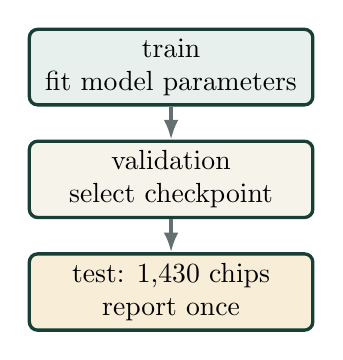
\begin{tikzpicture}[
        node distance=0.42cm,
        stage/.style={draw=forest,very thick,rounded corners=3pt,
          minimum width=3.6cm,minimum height=0.78cm,align=center},
        arr/.style={-{Latex[length=2.5mm]},very thick,draw=muted}
      ]
        \node[stage,fill=palegreen] (train) {train\\fit model parameters};
        \node[stage,fill=paper,below=of train] (val) {validation\\select checkpoint};
        \node[stage,fill=palegold,below=of val] (test) {test: 1,430 chips\\report once};
        \draw[arr] (train) -- (val);
        \draw[arr] (val) -- (test);
      \end{tikzpicture}
    \end{column}
    \begin{column}{0.41\textwidth}
      \begin{block}{Fair comparison}
        \begin{itemize}
          \item Common probability threshold: \textbf{0.60}
          \item Boundary evaluation tolerance:\\[-0.1em]
            \textbf{2 pixels ($\approx$20 m)}
          \item Same 1,430 test chips for all models
        \end{itemize}
      \end{block}
      \vspace{0.45em}
      \begin{block}{Metrics}
        \textbf{mIoU}: region overlap\\[0.35em]
        \textbf{Boundary IoU}: overlap of predicted and target boundary bands
      \end{block}
    \end{column}
  \end{columns}
\end{frame}

\begin{frame}{Test result: explicit boundary prediction gives the best BIoU}
  \begin{columns}[T,onlytextwidth]
    \begin{column}{0.52\textwidth}
      \centering
      \resizebox{\linewidth}{!}{%
      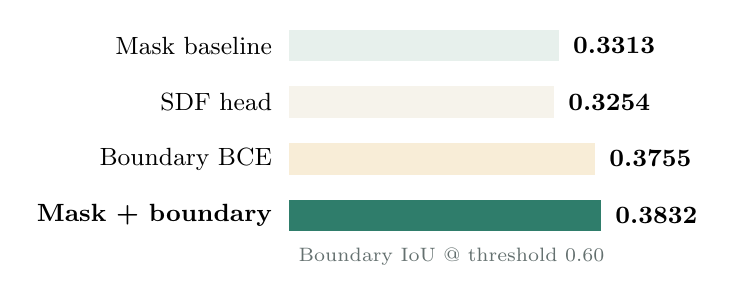
\begin{tikzpicture}[x=0.45cm,y=0.72cm]
        \node[anchor=east,font=\small] at (0,1.80) {Mask baseline};
        \node[anchor=east,font=\small] at (0,0.80) {SDF head};
        \node[anchor=east,font=\small] at (0,-0.20) {Boundary BCE};
        \node[anchor=east,font=\small\bfseries] at (0,-1.20) {Mask + boundary};
        \fill[palegreen] (0.2,1.52) rectangle (7.82,2.08);
        \fill[paper] (0.2,0.52) rectangle (7.68,1.08);
        \fill[palegold] (0.2,-0.48) rectangle (8.84,0.08);
        \fill[leaf] (0.2,-1.48) rectangle (9.01,-0.92);
        \node[anchor=west,font=\small\bfseries] at (7.95,1.80) {0.3313};
        \node[anchor=west,font=\small\bfseries] at (7.81,0.80) {0.3254};
        \node[anchor=west,font=\small\bfseries] at (8.97,-0.20) {0.3755};
        \node[anchor=west,font=\small\bfseries] at (9.14,-1.20) {0.3832};
        \node[anchor=west,font=\scriptsize,text=muted] at (0.2,-1.92)
          {Boundary IoU @ threshold 0.60};
      \end{tikzpicture}
      }
    \end{column}
    \begin{column}{0.44\textwidth}
      \footnotesize
      \setlength{\tabcolsep}{5pt}
      \begin{tabular}{@{}lrr@{}}
        \toprule
        Method & mIoU & BIoU \\
        \midrule
        Baseline & .6572 & .3313 \\
        SDF head & .6500 & .3254 \\
        Boundary BCE & \textbf{.6675} & .3755 \\
        \textbf{Mask + boundary} & .6634 & \textbf{.3832} \\
        \bottomrule
      \end{tabular}
      \vspace{0.6em}
      \begin{block}{Main test finding}
        The explicit boundary head adds \textbf{+0.77 pp BIoU} over Boundary BCE alone; Boundary BCE alone keeps the highest mIoU.
      \end{block}
    \end{column}
  \end{columns}
\end{frame}

\begin{frame}{The boundary head helps; the distance head does not}
  \begin{columns}[T,onlytextwidth]
    \begin{column}{0.48\textwidth}
      \begin{block}{All four test checkpoints}
        \begin{tabular}{@{}lcc@{}}
          \toprule
          Test @ 0.60 & mIoU & BIoU \\
          \midrule
          Baseline & .6572 & .3313 \\
          SDF head & .6500 & .3254 \\
          Boundary BCE & \textbf{.6675} & .3755 \\
          \textbf{Mask + boundary} & .6634 & \textbf{.3832} \\
          \bottomrule
        \end{tabular}
      \end{block}
    \end{column}
    \begin{column}{0.48\textwidth}
      \begin{block}{What changed}
        \textbf{Distance regression}\\
        Indirectly modifies shared features; no test gain.

        \vspace{0.45em}
        \textbf{Boundary-weighted mask loss}\\
        Directly changes mask gradients; $+4.42$ pp BIoU.

        \vspace{0.45em}
        \textbf{Explicit boundary head}\\
        Adds a focused border task; another $+0.77$ pp BIoU.
      \end{block}
    \end{column}
  \end{columns}
  \vspace{0.7em}
  \centering
  \pill{palegold}{The auxiliary target matters: predicting borders is more useful than regressing distance.}
\end{frame}

\begin{frame}{Qualitative comparison on the same Austria chip}
  \centering
  \begin{minipage}[t]{0.29\textwidth}
    \centering
    \parbox[c][1.7em][c]{\linewidth}{\centering\scriptsize\bfseries Sentinel-2 RGB}\par
    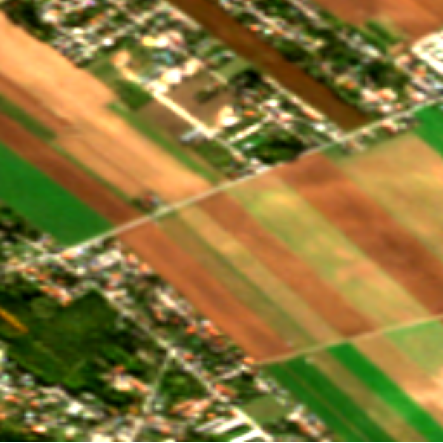
\includegraphics[width=\linewidth,height=0.27\textheight,keepaspectratio]
      {../Visualizations/sample_austria_g83_00040_14/rgb.png}
  \end{minipage}
  \hfill
  \begin{minipage}[t]{0.29\textwidth}
    \centering
    \parbox[c][1.7em][c]{\linewidth}{\centering\scriptsize\bfseries Ground truth}\par
    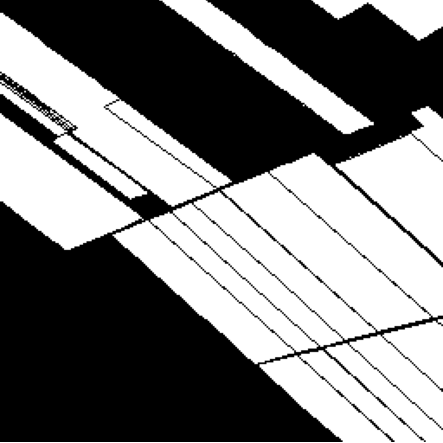
\includegraphics[width=\linewidth,height=0.27\textheight,keepaspectratio]
      {../Visualizations/sample_austria_g83_00040_14/ground_truth_mask.png}
  \end{minipage}
  \hfill
  \begin{minipage}[t]{0.29\textwidth}
    \centering
    \parbox[c][1.7em][c]{\linewidth}{\centering\scriptsize\bfseries Baseline}\par
    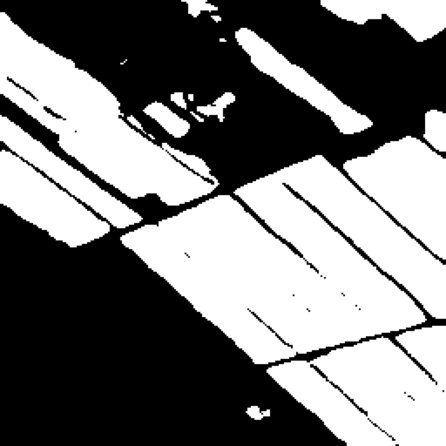
\includegraphics[width=\linewidth,height=0.27\textheight,keepaspectratio]
      {../Visualizations/presentation_comparison/baseline_mask.png}
  \end{minipage}

  \vspace{0.35em}

  \begin{minipage}[t]{0.29\textwidth}
    \centering
    \parbox[c][2.0em][c]{\linewidth}{\centering\scriptsize\bfseries SDF auxiliary head}\par
    
\includegraphics[width=\linewidth,height=0.27\textheight,keepaspectratio]
      {../Visualizations/presentation_comparison/sdf_head_mask.png}
  \end{minipage}
  \hfill
  \begin{minipage}[t]{0.29\textwidth}
    \centering
    \parbox[c][2.0em][c]{\linewidth}{\centering\scriptsize\bfseries Boundary BCE}\par
    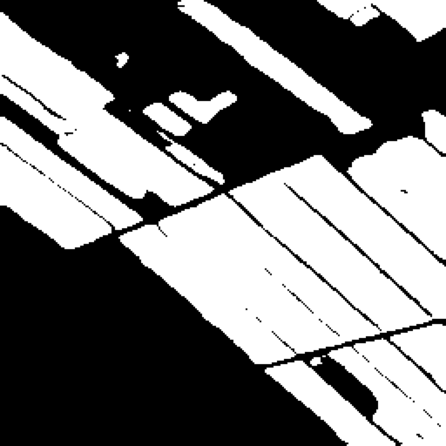
\includegraphics[width=\linewidth,height=0.27\textheight,keepaspectratio]
      {../Visualizations/presentation_comparison/boundary_bce_mask.png}
  \end{minipage}
  \hfill
  \begin{minipage}[t]{0.29\textwidth}
    \centering
    \parbox[c][2.0em][c]{\linewidth}{\centering\scriptsize\bfseries Mask + boundary heads}\par
    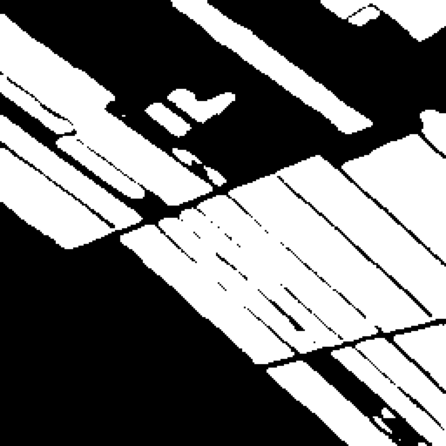
\includegraphics[width=\linewidth,height=0.27\textheight,keepaspectratio]
      {../Visualizations/presentation_comparison/mask_boundary_heads_mask.png}
  \end{minipage}

  \vspace{0.35em}
  {\scriptsize Same image and probability threshold (0.60) for every prediction.}
  \source{FTW validation chip \texttt{austria/g83\_00040\_14}; predictions generated in this project.}
\end{frame}

\begin{frame}{Conclusion and outlook}
  \begin{columns}[T,onlytextwidth]
    \begin{column}{0.58\textwidth}
      \begin{block}{Takeaway}
        Direct boundary supervision is more effective than auxiliary signed-distance regression.
      \end{block}
      \vspace{0.55em}
      \begin{itemize}
        \item Boundary BCE: $0.3313 \rightarrow 0.3755$ BIoU (\textbf{+4.42 pp})
        \item Adding the boundary head reaches \textbf{0.3832 BIoU} (\textbf{+5.19 pp})
        \item New model mIoU is $0.6634$, still $+0.62$ pp above baseline
        \item The SDF regression head does not improve the test checkpoint
      \end{itemize}
    \end{column}
    \begin{column}{0.38\textwidth}
      \begin{block}{Next steps}
        \begin{itemize}
          \item repeat with multiple random seeds
          \item report per-country performance
          \item test instance-separation post-processing
          \item study learned boundary calibration
        \end{itemize}
      \end{block}
    \end{column}
  \end{columns}
  \vspace{0.65em}
  \centering
  \pill{palegold}{Best boundary model: boundary-weighted mask loss + explicit boundary head.}
\end{frame}

\appendix

\begin{frame}{Backup: threshold sensitivity on the test set}
  \centering
  \small
  \setlength{\tabcolsep}{8pt}
  \begin{tabular}{@{}lcccccccc@{}}
    \toprule
    & \multicolumn{2}{c}{0.40} & \multicolumn{2}{c}{0.50}
    & \multicolumn{2}{c}{0.60} & \multicolumn{2}{c}{0.70} \\
    \cmidrule(lr){2-3}\cmidrule(lr){4-5}\cmidrule(lr){6-7}\cmidrule(lr){8-9}
    Method & mIoU & BIoU & mIoU & BIoU & mIoU & BIoU & mIoU & BIoU \\
    \midrule
    Baseline & .6593 & .3049 & .6587 & .3199 & .6572 & .3313 & .6506 & .3359 \\
    2-head SDF & .6554 & .3017 & .6528 & .3153 & .6500 & .3254 & .6369 & .3246 \\
    Boundary BCE & .6706 & .3364 & .6731 & .3618 & .6675 & .3755 & .6520 & .3682 \\
    Mask + boundary & .6717 & \textbf{.3499} & .6685 & \textbf{.3705} & .6634 & \textbf{.3832} & .6467 & \textbf{.3715} \\
    \bottomrule
  \end{tabular}

  \vspace{0.9em}
  \begin{block}{Why the main talk uses 0.60}
    It is a single common operating point for all four models. The new model has the best Boundary IoU at every tested threshold.
  \end{block}
\end{frame}

\begin{frame}{Backup: exact objectives}
  \begin{columns}[T,onlytextwidth]
    \begin{column}{0.48\textwidth}
      \begin{block}{Boundary BCE}
        \[
          \mathcal{L}_{BBCE}
          = \mathcal{L}_{WBCE}(z_M,Y)
          + \mathcal{L}_{Dice}
        \]
        \small One mask output; $\alpha=20$ and $\sigma=0.12$ define the pixel weights.
      \end{block}
    \end{column}
    \begin{column}{0.48\textwidth}
      \begin{block}{Mask + boundary heads}
        \[
          \mathcal{L}_{M+B}
          = \mathcal{L}_{WBCE}
          + \mathcal{L}_{Dice}
          + 2\mathcal{L}^{bal}_{BCE}(z_B,B)
        \]
        \small Two active outputs; the explicit boundary term has weight 2.
      \end{block}
    \end{column}
  \end{columns}
  \vspace{0.75em}
  \begin{block}{How the boundary target is formed}
    $B_i=\mathbf{1}[|D_i|\leq0.12]$. The precomputed distance target constructs the weights and boundary labels; the final model predicts only the mask and boundary maps.
  \end{block}
\end{frame}

\begin{frame}{Backup: references}
  \footnotesize
  \begin{thebibliography}{9}
    \bibitem{ftw}
      H. Kerner et al.
      \newblock \emph{Fields of The World: A Machine Learning Benchmark Dataset for Global Agricultural Field Boundary Segmentation}.
      \newblock AAAI, 2025.

    \bibitem{unet}
      O. Ronneberger, P. Fischer, and T. Brox.
      \newblock \emph{U-Net: Convolutional Networks for Biomedical Image Segmentation}.
      \newblock MICCAI, 2015.

    \bibitem{boundary}
      H. Kervadec et al.
      \newblock \emph{Boundary Loss for Highly Unbalanced Segmentation}.
      \newblock MIDL, 2019; extended in Medical Image Analysis, 2021.
  \end{thebibliography}

  \vspace{0.8em}
  \small
  All prediction panels and project diagrams were generated from this repository; no external figures are reproduced.
\end{frame}

\end{document}
